\documentclass[a4paper,12pt]{report} % добавить leqno в [] для нумерации слева

%%% Работа с русским языком
\usepackage{cmap}					% поиск в PDF
\usepackage{mathtext} 				% русские буквы в формулах
\usepackage[T2A]{fontenc}			% кодировка
\usepackage[utf8]{inputenc}			% кодировка исходного текста
\usepackage[english,russian]{babel}	% локализация и переносы

%%% Дополнительная работа с математикой
\usepackage{amsmath,amsfonts,amssymb,amsthm,mathtools} % AMS
\usepackage{icomma} % "Умная" запятая: $0,2$ --- число, $0, 2$ --- перечисление

%% Номера формул
\mathtoolsset{showonlyrefs=true} % Показывать номера только у тех формул, на которые есть \eqref{} в тексте.

%% Шрифты
\usepackage{euscript}	 % Шрифт Евклид
\usepackage{mathrsfs} % Красивый матшрифт

%% Свои команды
\DeclareMathOperator{\sgn}{\mathop{sgn}}

%\setlength\parindent{0ex}
%\setlength\parskip{0.3cm}

%%% Заголовок
\author{Волков Павел А-14-19}
\title{Типовой расчет №14 по численным методам Вариант 3}
\date{\today}

\usepackage{graphicx}

\begin{document} % конец преамбулы, начало документа

\maketitle

\newpage
\section*{Задание}

Функция $y = y(x)$ задана таблицей своих значений. Применяя метод наименьших квадратов, проблизить ее функцией вида $\Phi(x) = a\varphi_0(x) + b\varphi_1(x)$. Определить величину среднеквадратичной погрешности. Построить на одном чертеже точечный график исходных данных и график функции $\Phi(x)$
\[
\begin{tabular}{ | c | c | c | c | c | c | c |}
	\hline
	$x$ & 2.3 & 4.1 & 4.6 & 4.8 & 5.8 & 6.2 \\ \hline
	$y$ & -0.298 & 0.192 & -0.594 & -0.954 & -1.112 & -0.216 \\ \hline
\end{tabular}
\]
$\varphi_0(x) = \sin{x}$, $\varphi_1(x) = \sin{2x}$

\section*{Решение}

Запишем нормальную систему метода наименьших квадратов:
\[
	\left\{
		\begin{aligned}
		s_0a + s_1b = d_0  \\
		s_1a + s_2b = d_1 \\
		\end{aligned}
	\right.
\]
Где $d_k = \sum\limits_{i=0}^n f_i\varphi_k(x_i)$, $s_0 = \sum\limits_{i=0}^n \varphi_0(x_i)^2$, $s_1 =  \sum\limits_{i=0}^n \varphi_0(x_i)\varphi_1(x_i)$ и $s_2 =  \sum\limits_{i=0}^n \varphi_1(x_i)^2$

Решением этой системы будут коэффициенты: $a = 0.79989674$ и $b = 0.90003346$

Тогда приближающая функция $\Phi(x) = 0.79989674\sin{x} +  0.90003346\sin{2x}$ имеет среднеквадратичную погрешность: $\sigma(\Phi(x), f) = 0.000274859$, что подтверждается графиком:

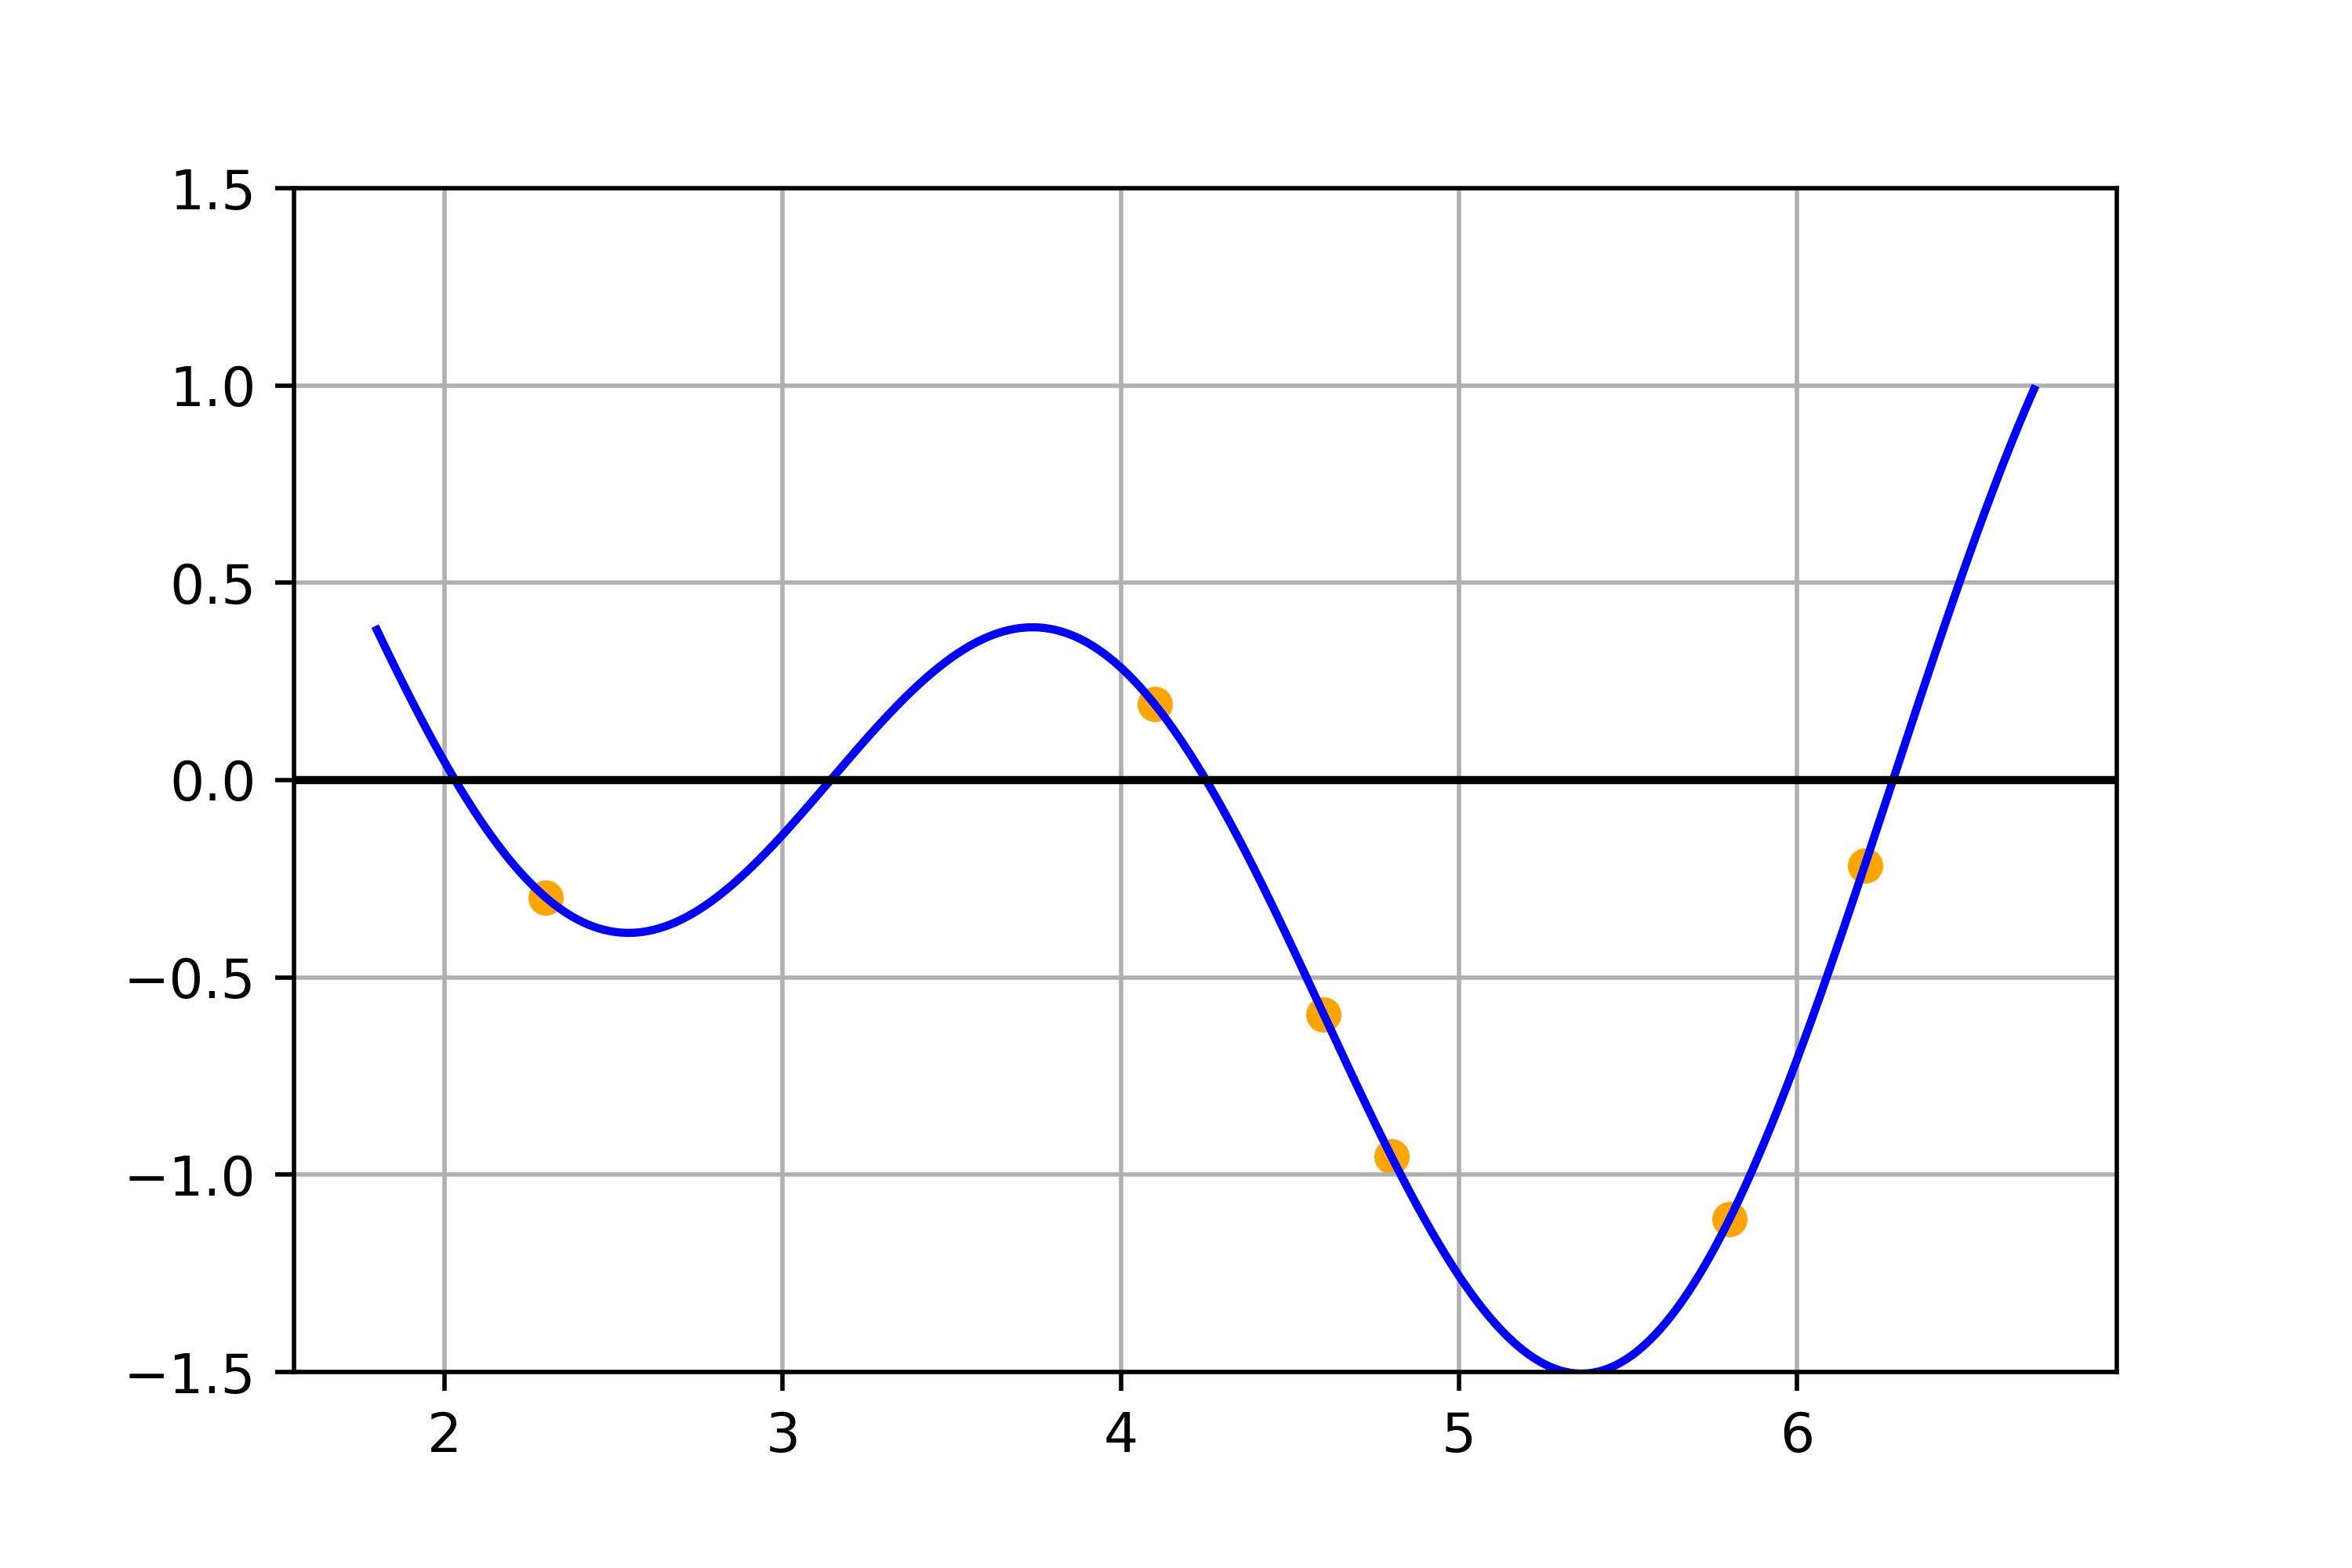
\includegraphics[height=7cm]{regular_calc_14.png}

\end{document}